\chapter{Lecture 2}

This lecture is about \texttt{Model Selection [CV, Bootstrap, Cp, AIC, BIC, ROC]} where chapter
\texttt{ESL Chapter 7 and 9.2.5. You may safely skip sections 7.8 and 7.9} should be looked upon.

\begin{itemize}
  \item Model Complexity
  \begin{itemize}
    \item Bias, variance, overfitting and underfitting
  \end{itemize}
  \item Model Selection
  \begin{itemize}
    \item Methods for selecting an appropriate model from an ensemble of candidates.
        \begin{itemize}
          \item Training, test and validation set
          \item Cross-validation
          \item Methods based on information criteria
        \end{itemize}
  \end{itemize}
  \item Model Assessment
  \begin{itemize}
    \item Bootstrap
    \item Sensitivity, specificity and ROC curves
  \end{itemize}
\end{itemize}





\section{Chapter 7}

Bias Variance trade-off. The AIC and BIC and Cross-validation. Different Bootstrap methods

\section{Chapter 9}

Tree-Based method Spam Example.

\section{Model Complexity}

\begin{itemize}
  \item Overfitting and underfitting
  \item Regularization
  \item Bias and variance
\end{itemize}



\section{Overfitting and underfitting}

From lecture \cite[p.~7]{lecture2} then we know that we prefer a simple model and a model that work e.g. have low EPE.

So if a model is too simple, then Our data set will not be accurately described. Model assumptions are wrong.\\

And if it is too complex then The model becomes too flexible. We fit noise in data. We need lots of data to support such a model.

So we might wish to do regularization and there are two approaches

\begin{itemize}
  \item Bayesian prior to $\beta$
  \item Penalty to models with large $\beta$
\end{itemize}

From lecture \cite[p.~18]{lecture2} then we can use Ridge Regression. We can use a flexible model and avoid overfitting via regularization.

With the simple solution

\[
    \beta_{\text{ridge}} = (\bm{X}^T\bm{X} + \lambda \bm{I})^{-1} \bm{X}^T\bm{y}
\]

where regularization parameter $\lambda$.

\begin{itemize}
  \item $\lambda = 0$ gives $\beta_{\text{ridge}} = \beta_{\text{OLS}}$
      \begin{itemize}
        \item No bias
        \item High Variance
      \end{itemize}
  \item $\lambda \rightarrow 0$ gives $\beta_{\text{ridge}} \rightarrow 0$
      \begin{itemize}
        \item High bias
        \item No Variance
      \end{itemize}
\end{itemize}


\section{Regularization}

\cite[p.~17]{lecture2}

From wiki:\footnote{\href{https://www.wikiwand.com/en/Regularization_(mathematics)}{regularization mathematics}}

Early stopping can be viewed as regularization in time. Intuitively, a training procedure like gradient descent will tend to learn more and more complex functions as the number of iterations increases. By regularizing on time, the complexity of the model can be controlled, improving generalization.

In practice, early stopping is implemented by training on a training set and measuring accuracy on a statistically independent validation set. The model is trained until performance on the validation set no longer improves. The model is then tested on a testing set.

\section{Bias Variance trade-off}

\textbf{Model selection:} estimating the performance of different models in order to choose the best one.

\textbf{Model assessment:} having chosen a final model, estimating its prediction error (generalization error) on new data.

If we are in a data-rich situation, the best approach for both problems is to randomly divide the dataset into three parts: a training set, a validation set, and a test set. The training set is used to fit the models; the validation set is used to estimate prediction error for model selection; the test set is used for assessment of the generalization error of the final chosen model.
Ideally, the test set should be kept in a “vault,” and be brought out only at the end of the data analysis. Suppose instead that we use the test-set repeatedly, choosing the model with smallest test-set error. Then the test set error of the final chosen model will underestimate the true test error, sometimes substantially \cite[p.~222]{friedman2016elements}\\

If a model is not complex enough it produce \textbf{underfit} models, that can't learn the signal from the data.\\

But if a model is too comples, it produce \textbf{overfit} models that memorize the noise instead of the signal

%https://elitedatascience.com/bias-variance-tradeoff

\subsection{Bias Variance Decomposition}

Assume that $Y = f(X) + \varepsilon$ and $E(\varepsilon) = 0$ and $Var(\varepsilon) = \sigma^2_\varepsilon$

Then we have

\begin{equation}
  \begin{split}
     Err(x_0) =  & \: E[(Y- \hat{f}(x_0))^2 | X = x_0] \\
       =& \: \sigma^2_\varepsilon + [E \hat{f}(x_0) - f(x_0)]^2 + E[\hat{f}(x_0) - E\hat{f}(x_0)]^2 \\
       =& \: \sigma_\varepsilon^2 + \text{Bias}^2 (\hat{f}(x_0)) + \text{Var}(\hat{f}(x_0)) \\
       =& \: \text{Irreducible Error} + \text{Bias}^2 + \text{Variance}
  \end{split}
\end{equation}

It does not depend at all upon our choice of model
but simply represents the intrinsic difficulty of the problem. We cannot make this term any larger or smaller by selecting one model over another, unless $\sigma_\varepsilon^2 = 0$

The second term $ [E \hat{f}(x_0) - f(x_0)]^2 $, squared bias, tells us how much the average values of models trained on different training datasets differ compared to the true mean of the data $\hat{f}(x_0)$

The last term $E[\hat{f}(x_0) - E\hat{f}(x_0)]^2$ is the variance term. It tells us how much the model wiggles when trained on different sets of training data. That is when you train models on $N$ different sets of training data and the models are nearly the same, this term is small.

\begin{figure}[H]
  \centering
  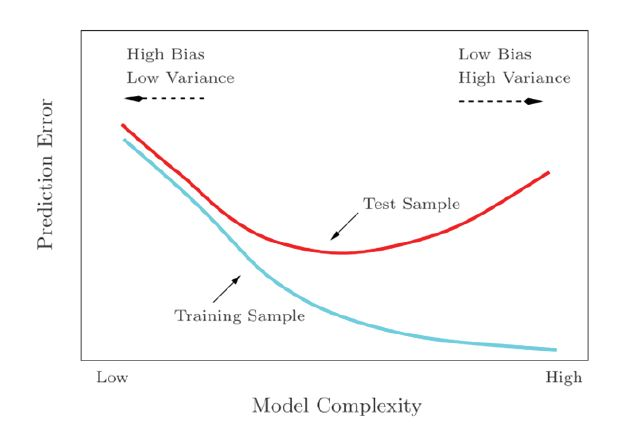
\includegraphics[width=0.9\textwidth]{modelcomplexity}
  \caption{Bias and variance the model complexity}\label{fig:modelcomplexity}
\end{figure}

\section{Cross-Validation}

The more complex the model, the better we will fit the training data.
Often we overfit to the training data.\\

Overfit models can perform poorly on test data - high variance.\\


Underfit models can perform poorly on test data - high bias.\\

As discussed, we perform \textbf{Model Selection} and \textbf{Model assessment}. For both of these purposes, the best approach is to evaluate the procedure on an independent test set. \cite[p.~]{lecture2}



Often there is insufficient data to create a separate validation and test set. In this instance use cross validation instead.\cite[p.~30]{lecture2}

\begin{itemize}
  \item The primary method for estimating a tuning parameter, e.g. $\lambda$
  \item No underlying assumptions
  \item Is simple, intuitive and easy to implement
\end{itemize}

Split randomized data in $K$ equal parts

\begin{figure}[H]
  \centering
  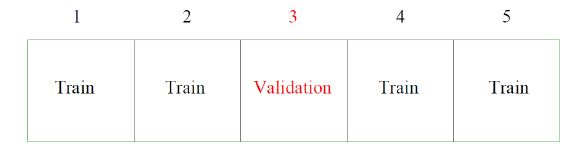
\includegraphics[width=0.9\textwidth]{splittingsetforCV}
\end{figure}

For each $k = 1, 2, ... , K$ fit the model for parameter $\lambda$ to the other $K-1$ parts, give $\hat{\beta}^{\neg k}(\lambda)$ and compute its error in predicting the \textit{k}th part:

\[
    E_k(\lambda) = \sum_{i \in k \text{th part}} (y_i - X_i \hat{\beta}^{\neg k}(\lambda))^2
\]

This gives the cross-validation error

\[
    CV ( \lambda) = \frac{1}{K} \sum_{k=1}^{K} E_k(\lambda)
\]

Do this for many values for $\lambda$ and choose the value of $\lambda$ that makes $CV(\lambda)$ smallest.

From \cite[p.~243]{friedman2016elements}, then to summarize, if the learning curve has a considerable slope at the given
training set size, five- or tenfold cross-validation will overestimate the true
prediction error. Whether this bias is a drawback in practice depends on
the objective. On the other hand, leave-one-out cross-validation has low
bias but can have high variance. Overall, five- or tenfold cross-validation
are recommended as a good compromise:\\

From lecture \cite[p.~32]{lecture2} we use the \textbf{one standard error rule}, where we choose the smallest model whose error is no more than one standard error above the error of the best model.
This compensates that the CV procedure chooses somewhat too complex models.

Consider a classification problem with a large number of predictors, as may arise, for example, in genomic or proteomic applications. A typical strategy for analysis might be as follows:

\begin{itemize}
  \item Screen the predictors: find a subset of “good” predictors that show fairly strong (univariate) correlation with the class labels
  \item Using just this subset of predictors, build a multivariate classifier.
  \item Use cross-validation to estimate the unknown tuning parameters and to estimate the prediction error of the final model.
\end{itemize}

\subsection{Considerations}

Observations are supposed to be independent. Otherwise
information will leak from validation set to training set and we
will overfit.

\begin{itemize}
  \item Permute data before splitting in folds - the data set might be sorted in some way.
  \item Normalize training data separately for each fold.
  \item Impute missing values separately for each training set.
  \item If observations are sampled in groups, let each group go into the same fold.
  \item Be extremely careful with data sampled from dynamic systems (time-dependent data).
  \item Be careful to perform ALL pre-processing within the CV folds.
\end{itemize} \cite[p.~34]{lecture2}\cite[p.~241-249]{friedman2016elements}

\subsection{Leave one out cross-validation}

Be careful using leave-one-out CV (K = N), the folds are too similar.
Use K = 5 or 10 as a good compromise between bias and variance.  \cite[p.~34]{lecture2}

\section{Information criteria}

\begin{itemize}
  \item Optimism and training error
  \item Information Criteria
\end{itemize}

\subsection{Optimism of the training error}

From lecture \cite[p.~37]{lecture2} and \cite[p.~228]{friedman2016elements} then the training error for OLS regression is

\[
    \frac{1}{N} \sum_{i=1}^{N} (y_i - x_i \hat{\beta})^2
\]

Think that we for each $x_i$ can get a new measurement $y_i^0$. What would the error for these new $y_i^0$ be? The in-sample-error

\[
    \frac{1}{N} \sum_{i=1}^{N} (y_i^0 - x_i \hat{\beta})^2
\]

Selecting the model with the smallest in-sample-error would be
an effective model selection tool.

The difference between the in-sample-error and the training-error
is called optimism. It is possible to show that quite generally

\[
    \frac{2}{N} \sum_{i=1}^{N} Cov(\hat{y}_i, y_i)
\]

The more we overfit data the greater $Cov(\hat{y}_i, y_i)$ will be and thereby increasing the optimism.\\

In the linear case with d variables and squared error loss we have expected optimism

\[
    \text{expected optimism} = d \sigma^2_e
\]

Therefore we have that

\[
    \text{expected in-sample-error} = \text{expected training-error} + 2 \frac{d}{N} \sigma^2_e
\]

the number d of inputs or basis functions we use, but decreases as the
training sample size increases from \cite[p.~230]{friedman2016elements}.

An obvious way to estimate prediction error is to estimate the optimism
and then add it to the training error

\subsection{CP-statistic}

Given a squared error loss and a model with d variables we can
calculate the so-called $C_p$-statistic

\[
    C_p = \overline{\text{err}} + 2 \frac{d}{N} \sigma^2_e
\]

where

\[
    \overline{\text{err}} = \frac{1}{N} \sum_{i=1}^{N} L(y_i, \hat{f}(x_i))
\]

Using this metric we can select the best model by choosing the model
that minimizes $C_p$.\\

Expected training error, use the actual training error

\[
    \frac{1}{N} \sum_{i=1}^{N} (y_i - x_i \hat{\beta})^2
\]

Noise variance, use the mean squared error (MSE) of low bias model (OLS or KNN) as the estimate $\hat{\sigma}^2_e$ from lecture \cite[p.~39]{lecture2}



\subsection{AIC}

To use AIC for model selection, we simply choose the model giving smallest AIC over the set of models considered. \cite[p.~231]{friedman2016elements}
AIC uses a log-likelihood loss function (logL) to estimate the error term (maximized log-likelihood)\cite[p.~40]{lecture2}

\[
    AIC = - \frac{2}{N} \log \text{L} + 2 \frac{d}{N}
\]

For the Gaussian case with a tuning parameter $\lambda$ we define

\[
    AIC(\lambda) = \overline{err}(\lambda) + 2 \frac{d(\lambda)}{N} \hat{\sigma}^2_e
\]

For the Gaussian model $C_p$ and AIC are identical. Where $d(\lambda)$ is the effective number of parameters in the model tuned with $\lambda$

I Often leave-one-out cross-validation and AIC tend to choose
models which are too complex. \cite[p.~45]{lecture2}

\subsection{Effective number of parameters}

From \cite[p.~232]{friedman2016elements}, then the concept of “number of parameters” can be generalized, especially to models where regularization is used in the fitting.

For a linear fitting method then from lecture \cite[p.~41]{lecture2}

\[
    \hat{Y} = SY
\]

then we can calculate the effective number of parameters as

\[
    df(S) = trace(S)
\]

i.e. the sum of the diagonal elements of $S$.

Both OLS and ridge regression are linear fitting methods.



\subsection{BIC}

The Bayes Information Criterion, BIC, is like AIC based on a log
likelihood loss function. It is motivated from a Bayesian approach
selecting the model with the largest posterior probability. \cite[p.~42]{lecture2}

\[
    BIC = -2 \log \text{L} + \log(N) d
\]

Under the Gaussian model and squared error loss

\[
    BIC(\lambda) = \frac{N}{\hat{\sigma}^2_e} \left(
    \overline{err} (\lambda) + \log (N) \frac{d(\lambda)}{N} \hat{\sigma}^2_e \right)
\]

Again, select the model that has the lowest value.

BIC tends to penalize complex models more heavily, giving preference to simpler models in selection. As with AIC, $\sigma^2_\varepsilon$ is typically estimated by the mean square error of a low bias model. \cite[p.~233]{friedman2016elements}


For AIC and BIC, then for a given set of models:

\begin{itemize}
  \item As $n \rightarrow \infty$ the probability that BIC selects the correct model approaches one, whereas AIC tends to select a model which is too complex
  \item For small sample sizes BIC tends to select a model which is too simple
\end{itemize}

So, BIC is good for large models, while AIC is good for small models.






\section{Bootstrap Methods}

For the bootstrap method, look at lecture  \cite[p.~46]{lecture2} and book \cite[p.~249]{friedman2016elements}

Bootstrap is a general method for assessing statistical accuracy, furthermore the statistical bootstrap is also an absurdly simple and effective way of solving apparently hard problems.

\textbf{Note:}

If you don't have enough data to train your algorithm you can increase the size of your training set by (uniformly) randomly selecting items and duplicating them (with replacement).

Take a sample of the time of day that you wake up on Saturdays. Some Friday nights you have a few too many drinks, so you wake up early (but go back to bed). Other days you wake up at a normal time. Other days you sleep in.\\

\textbf{Here are the results:} [3.1, 4.8, 6.3, 6.4, 6.6, 7.3, 7.5, 7.7, 7.9, 10.1]\\

\textbf{What is the mean time that you wake up?} Well it's 6.8 (o'clock, or 6:48). A touch early for me.\\

How good a prediction is this of when you'll wake up next Saturday? Can you quantify how wrong you are likely to be?

It's a pretty small sample, and we're not sure of the distribution of the underlying process, so it might not be a good idea to use standard parametric statistical techniques.

Why don't we take a random sample of our sample, and calculate the mean and repeat this? This will give us an estimate of how bad our estimate is.

I did this several times, and the mean was between 5.98 and 7.8\\

Given a training set $Z = (z_1, z_2, ... , z_N)$ where $z_i = (x_i, y_i)$.

In figure \ref{fig:bootstrapmethod}, $S(\bm{Z})$ is any quantity computed from the data $\bm{Z}$, for example, the prediction at some input point. From the bootstrap sampling we can estimate any aspect of the distribution of $S(\bm{Z})$, for example, its
variance,

\[
    \hat{\text{Var}}[S(\bm{Z})] = \frac{1}{B-1} \sum_{b=1}^{B} (S(\bm{Z}^{*b})-\overline{S}^*)^2
\]
where

\[
    \overline{S}^* = \sum_{b} \frac{S(\bm{Z}^{*b})}{B}
\]

The variance of a parameter, S, is estimated by taking the variance
over B bootstrap replications (the value of the parameter for the
specific bootstrap samples).

\begin{figure}[H]
  \centering
  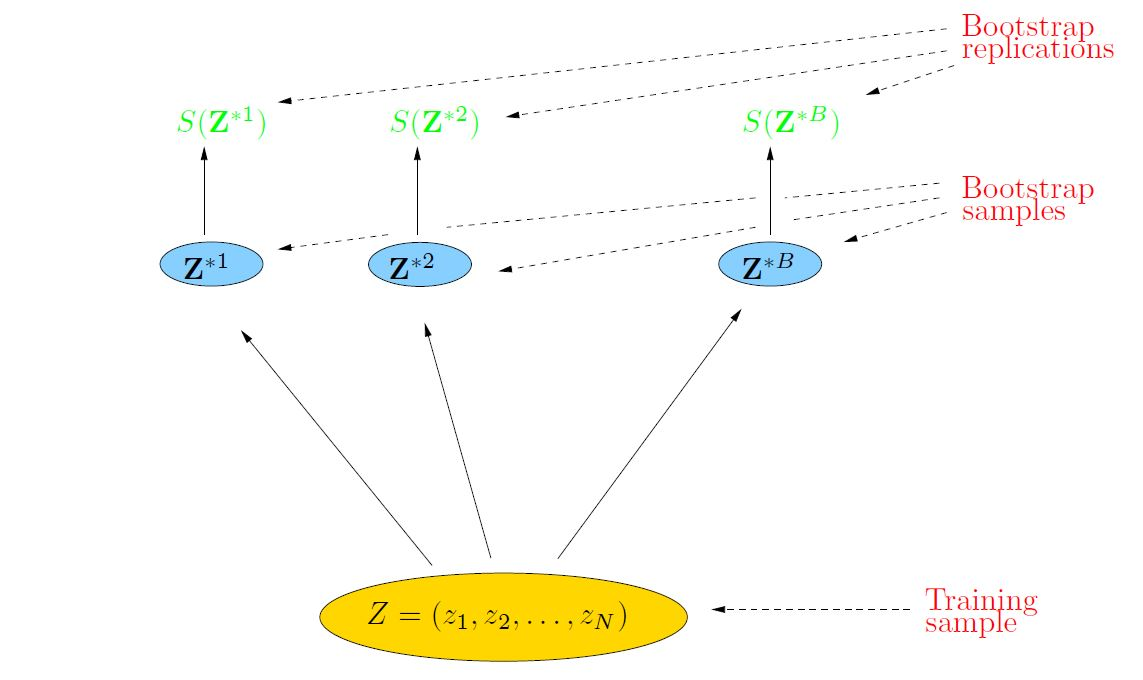
\includegraphics[width=0.9\textwidth]{bootstrapmethod}
  \caption{Schematic of the bootstrap process. We wish to assess the statistical accuracy of a quantity $S(\bm{Z})$ computed from our dataset. B training sets $Z^{*b}, b=1,...,B$ each of size $N$ are drawn with replacement from the original dataset. The quantity of interest $S(\bm{Z})$ is computed from each bootstrap training set, and the values $S(\bm{Z}^{*1}),...,S(\bm{Z}^{*B})$ are used to assess the statistical accuracy of $S(\bm{Z})$ }\label{fig:bootstrapmethod}
\end{figure}


\section{Classifier performance}


\subsection{Classifiers}


\subsection{LDA}
Find a linear combination $Z = a^T X$ such that the between-class variance is maximized relative to the within-class variance

\begin{figure}[H]
  \centering
  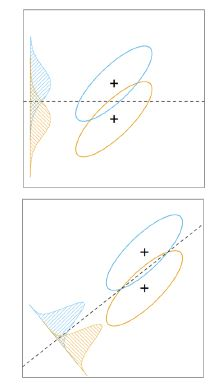
\includegraphics[height=0.5\textwidth]{FLLDA}
  \caption{Example of the Linear Discriminant Analysis}\label{fig:FLLDA}
\end{figure}

Maximize between-class variance $a^T \Sigma_B a$ where

\[
    \Sigma_B = \sum_{j=1}^{K} (\mu_j - \mu)^T(\mu_j - \mu)
\]

Minimize the within-class variance $a^T \Sigma_W a$ where

\[
    \Sigma_W = \sum_{j=1}^{K} \sum_{i=1}^{n_j} (X_{ij} -\mu_j)^T (X_{ij} -\mu_j)
\]

where the group mean is $u_j$ and total mean is $\mu$. Then the separating line is given by

\[
    \max\limits_a \frac{a^T \Sigma_B a}{a^T \Sigma_W a}
\]

from lecture \cite[p.~59]{lecture1}

\cite[p.~106-]{friedman2016elements}

\subsection{Confusion Matrix}

The confusion matrix have TP, FP, FN and TN, where

\begin{itemize}
  \item TP = True Positive which means hits
  \item FP = False Positive which means false alarm
  \item FN = False Negative which means misses
  \item TN = True Negative which means correct rejection
\end{itemize}

Then we have the

\begin{itemize}
  \item Sensitivity (TPR) which is Your method’s ability to identify positives
  \item Specificity (SPC) Your method’s ability to identify negatives
  \item Positive Predictive Value (PPV) Proportion of positives which are correctly classified
  \item Negative Predictive Value (NPV) Proportion of negatives which are correctly classified
  \item False Discovery Rate (FDR) Proportion of positives which are incorrectly classified
\end{itemize}

\subsection{ROC Curve}

Sensitivity and specificity changes as the cut-off value changes.

\begin{figure}[H]
  \centering
  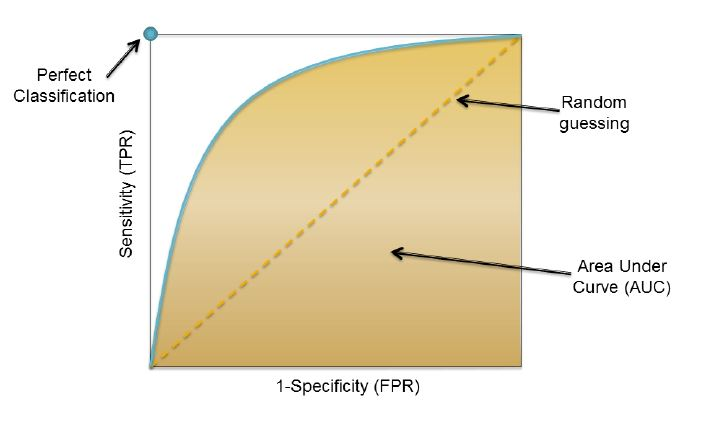
\includegraphics[width=0.9\textwidth]{ROCCURVE}
\end{figure}

\subsection{AUC}

Can we explicitly maximize AUC when creating models?

AUC is discrete, hard to optimize model parameters directly
w.r.t. AUC.

Most continuous methods such as maximum likelihood
corresponds well to AUC.

Regularization
Select regularization parameter based on AUC.

But use AUC with caution.\\

Assume you are segmentting a small part, 1\%, of an image (e.g. a
tumor in a mammography)

You have a large number of true negatives (TN) and the penalty for a segmentation twice as large as it should be?\\

Specificity = TN/(TN+FP) = 1mio/(1mio+10000) which is Specificity: 100\% => 99\%.\\

Result: AUC is very high, even though the segmentation is poor.
Interpret with caution when prevalence is off.


Summary

\begin{itemize}
  \item Over- and underfitting
  \item Model selection
  \begin{itemize}
    \item Traning/validation/test set
    \item Cross-validation
    \begin{itemize}
      \item One standard error rule
    \end{itemize}
    \item Information criterion
    \begin{itemize}
      \item $C_p$-statistics
      \item AIC
      \item BIC
    \end{itemize}
  \end{itemize}
  \item Model assessment
  \begin{itemize}
    \item Bootstrap
    \item Sensitivity vs specificity and ROC curves
    \item Confusion matrices
  \end{itemize}
\end{itemize}

